\subsection{Layers}
\label{sec:layers}

We start by analyzing layers in terms of size and compressibility, file and
directory counts, and layer directory depths.

\paragraph{Layer size}

\begin{figure}[t]
	\centering
		\begin{minipage}{0.24\textwidth}
			\centering
			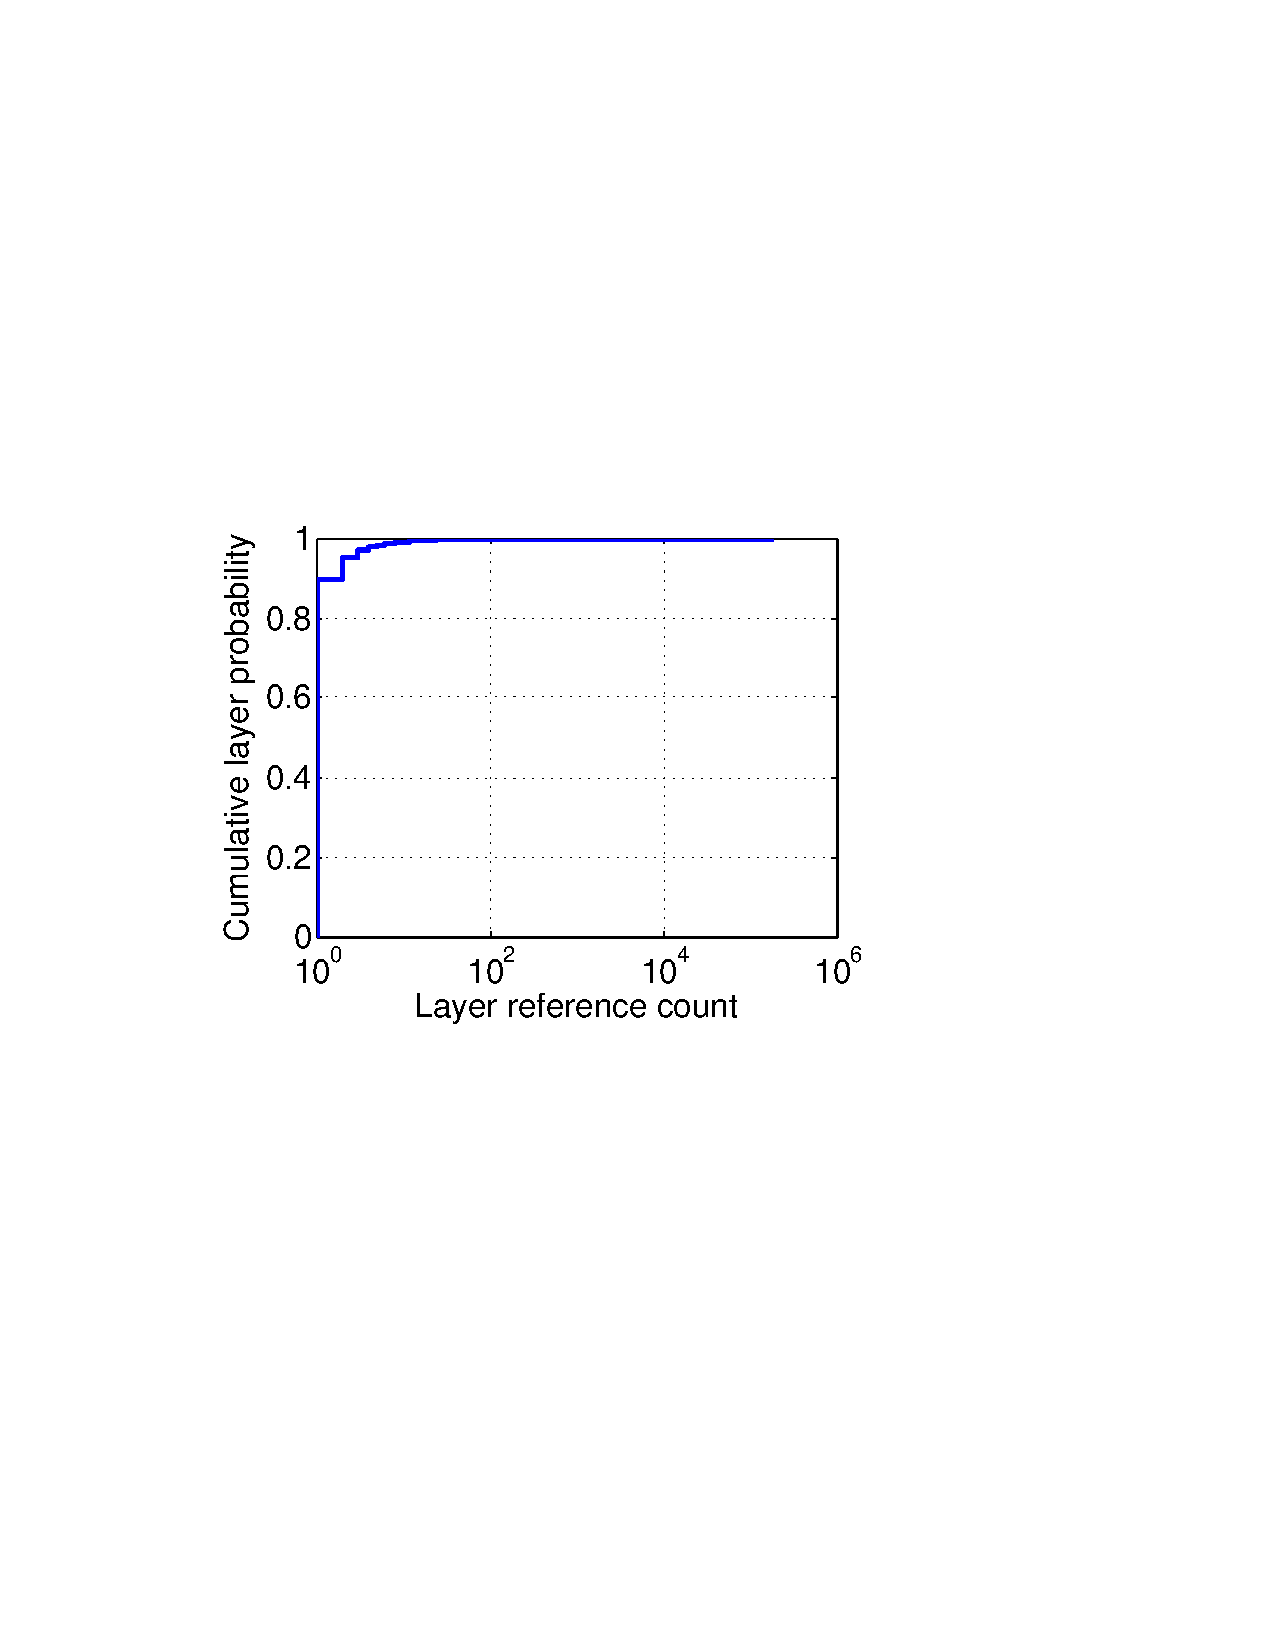
\includegraphics[width=1\textwidth]{graphs/shared-cnt-cdf.pdf}
			\caption{CDF of layer\\\ reference count.}
			\label{fig:ref_count}
		\end{minipage}
	\begin{minipage}{0.22\textwidth}
		\centering
		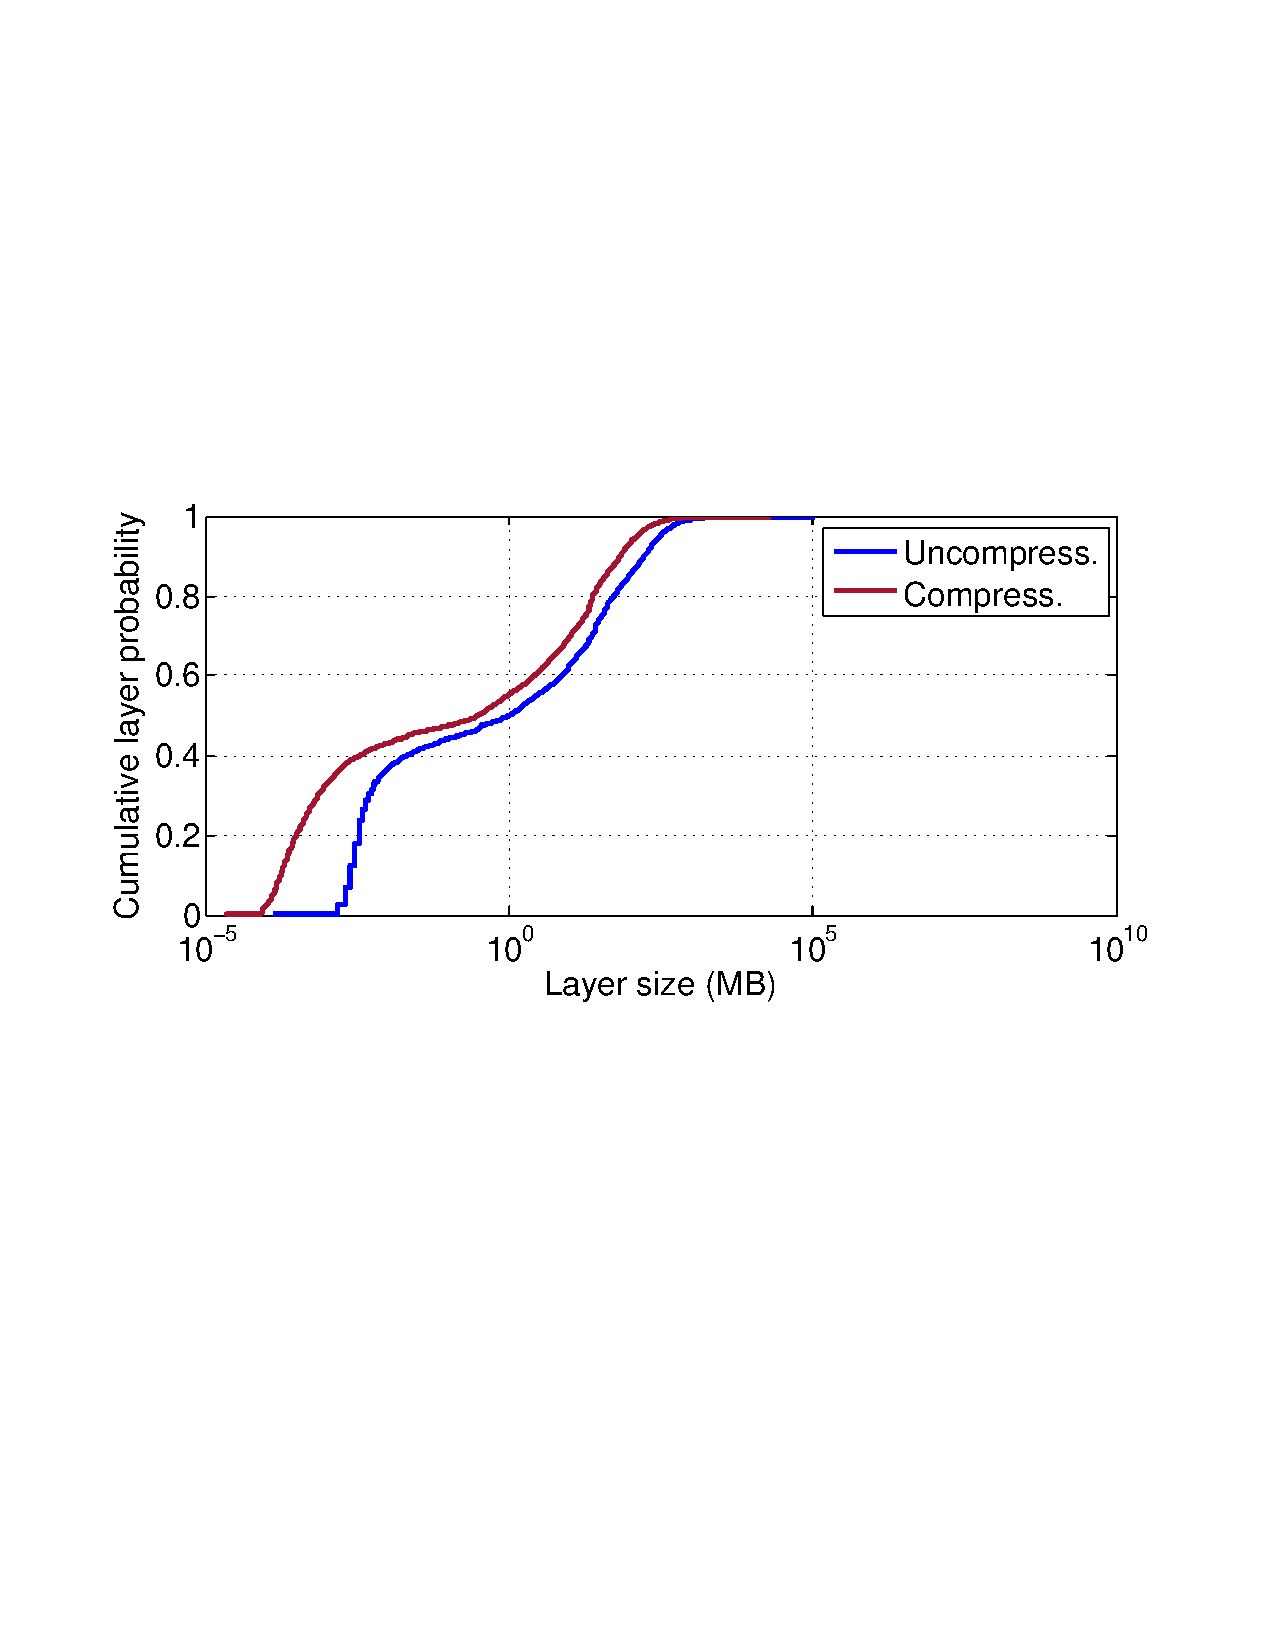
\includegraphics[width=1\textwidth]{graphs/layer-size-cdf.pdf}
		\caption{CDF of compress. and uncompress. layer size.}
		\label{fig:layer-size-cdf}
	\end{minipage}
\end{figure}


Recall that container image consists of multiple layers and each of these layer
is stored in Docker registry.
%
In figure~\ref{fig:layer-size-cdf} we show the compressed/uncompressed layer
size distribution.
%
We find that around 50\% of the layers are 1~MB in size and 90~\% of layers are
less than 64~MB in compressed format.
%
\emph{This finding is particularly useful for the Docker registry designers as
it shows that selective or popular layers can be cached in memory at the
registry side.}

%90\% of layers are less than 180 MB in uncompressed format
%
%As shown in , 90\% of layers are smaller than 64 MB


We decompressed the layer compressed gzip archival files and measured the
uncompressed layer size as shown in Figure~\ref{fig:layer-size-cdf}.
%
We see that 50\% of layers are smaller than 2 MB in uncompressed format and
90\% of layers are smaller than 170 MB in uncompressed format.
%
\emph{Compare with compressed layer size, we see that there are plenty of
redundant data in layers}

%We see that 90\% of the layers are smaller than 177~MB in uncompressed format
%and smaller than 63~MB in compressed format.
%%Interestingly, about half of the layers are smaller than 4~MB, independent of
%%the format.
%\nancomment{need check num}
%That means that the registry stores a large number of small layers
%which can benefit from compression.

%To analyze the frequencies, we zoom into the 0--128~MB range (see
%Figure~\ref{fig_hist_layer_size}).
%More than 1 million and 800,000 layers are smaller than 5~MB in compressed and
%uncompressed format, respectively. Beyond that, the frequency drops rapidly and
%we only see around 100,000 layers between 5~MB and 15~MB.

\paragraph{Compression ratio}

To understand how much redundant data is in each layer, we calculated the
compression ration as shown in Figure~\ref{fig:compress-ratio}.
%
We see that 80\% of layers have compression ratio less than 11 and 50\% of
layers have compression ratio less than 4.
%
\emph{High compression ratio shows the potential of compression while
distributing the container images.}

However, looking at Figure~\ref{fig:compress-ratio},
Figure~\ref{fig_hist_layer} we find that there are 3\% of layers for which the
compression ratio is around 1.
%
Doing compression and uncompression of such layers incur additional overhead at
docker engine side.
%
For such layers, we suggest not to do compression.
%
Docker engine can use a hybrid approach to compress only those layers which
yield better compression ratio.
%
\emph{This way users pulling such layers do not need to uncompress and will
experience reduction in container startup time.}

%\begin{figure}[!t]
%	\centering
%	\subfigure[CDF of layer depth]{\label{fig_reference_cnt_cdf}
%		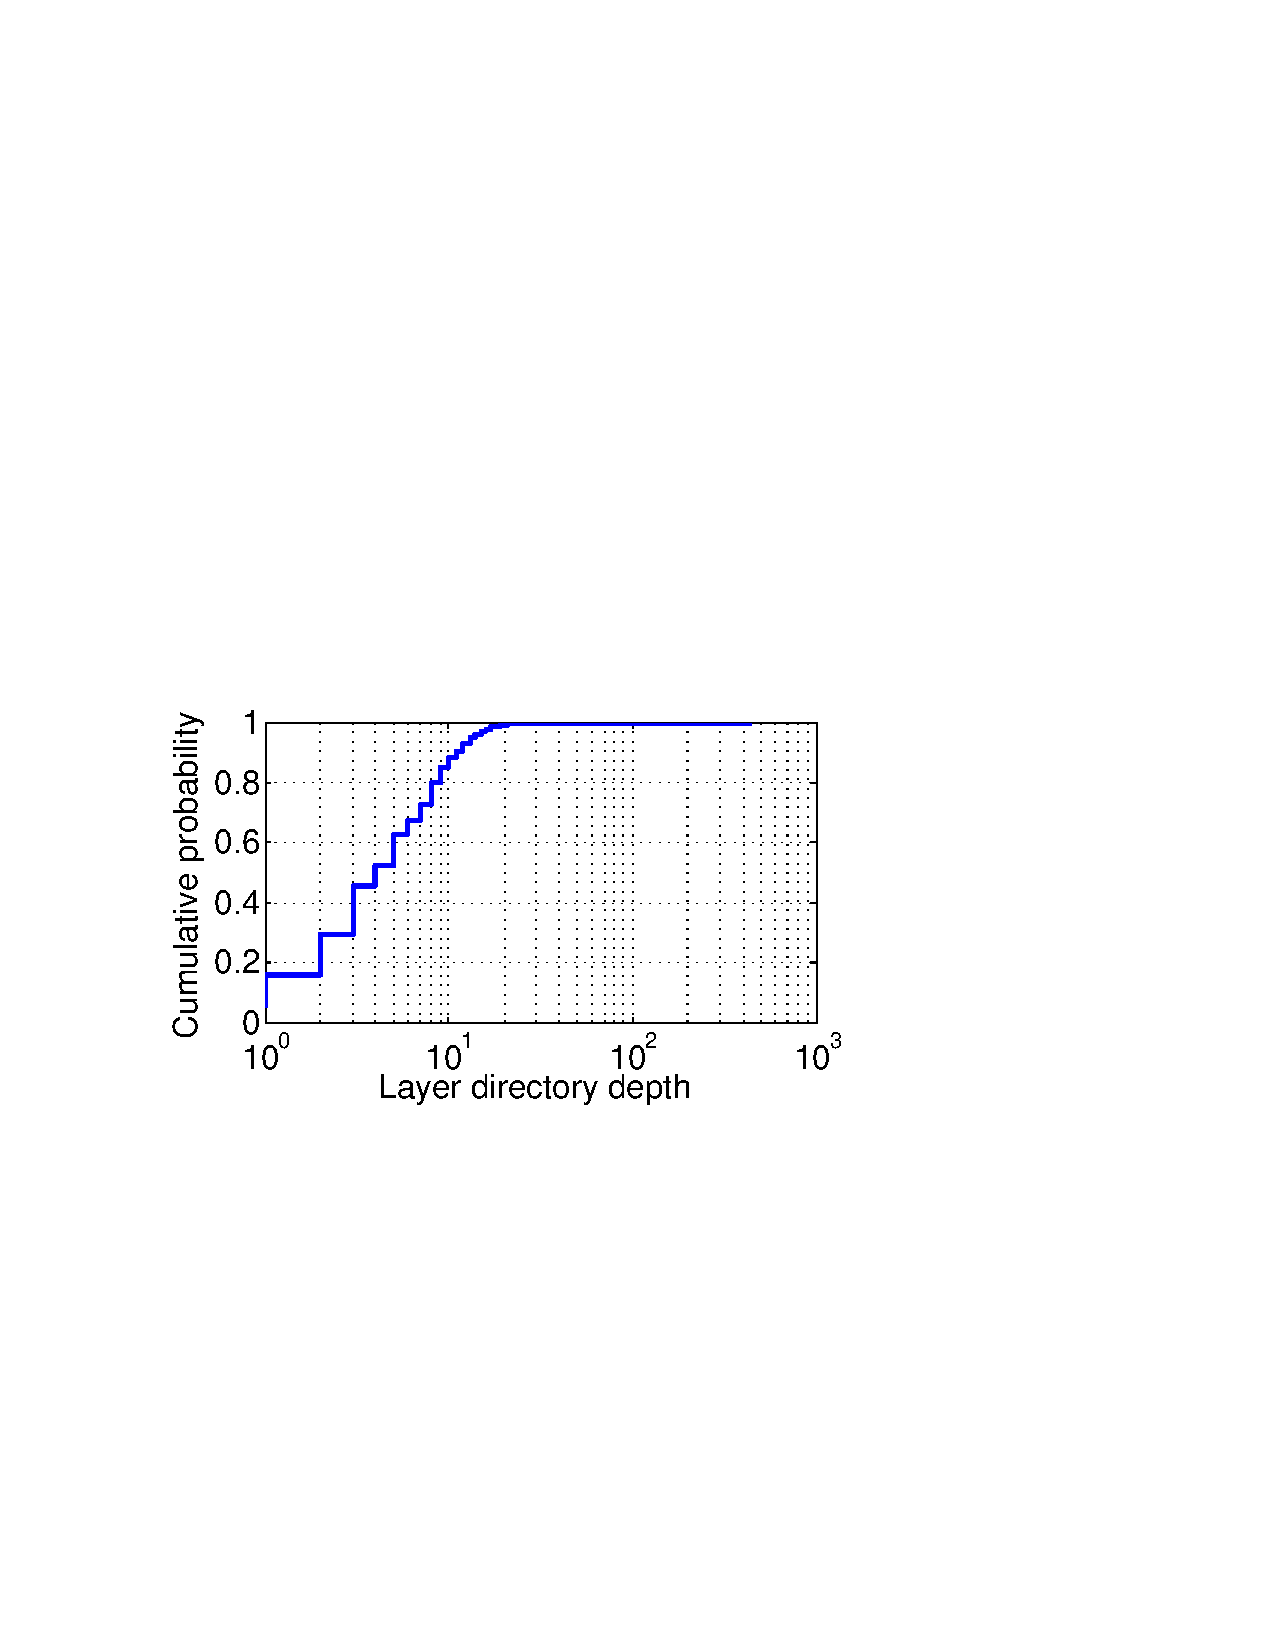
\includegraphics[width=0.21\textwidth]{graphs/layer-depth-cdf.pdf}%
%	}
%	\subfigure[Histogram of layer depth]{\label{fig_reference_cnt_pdf}
%		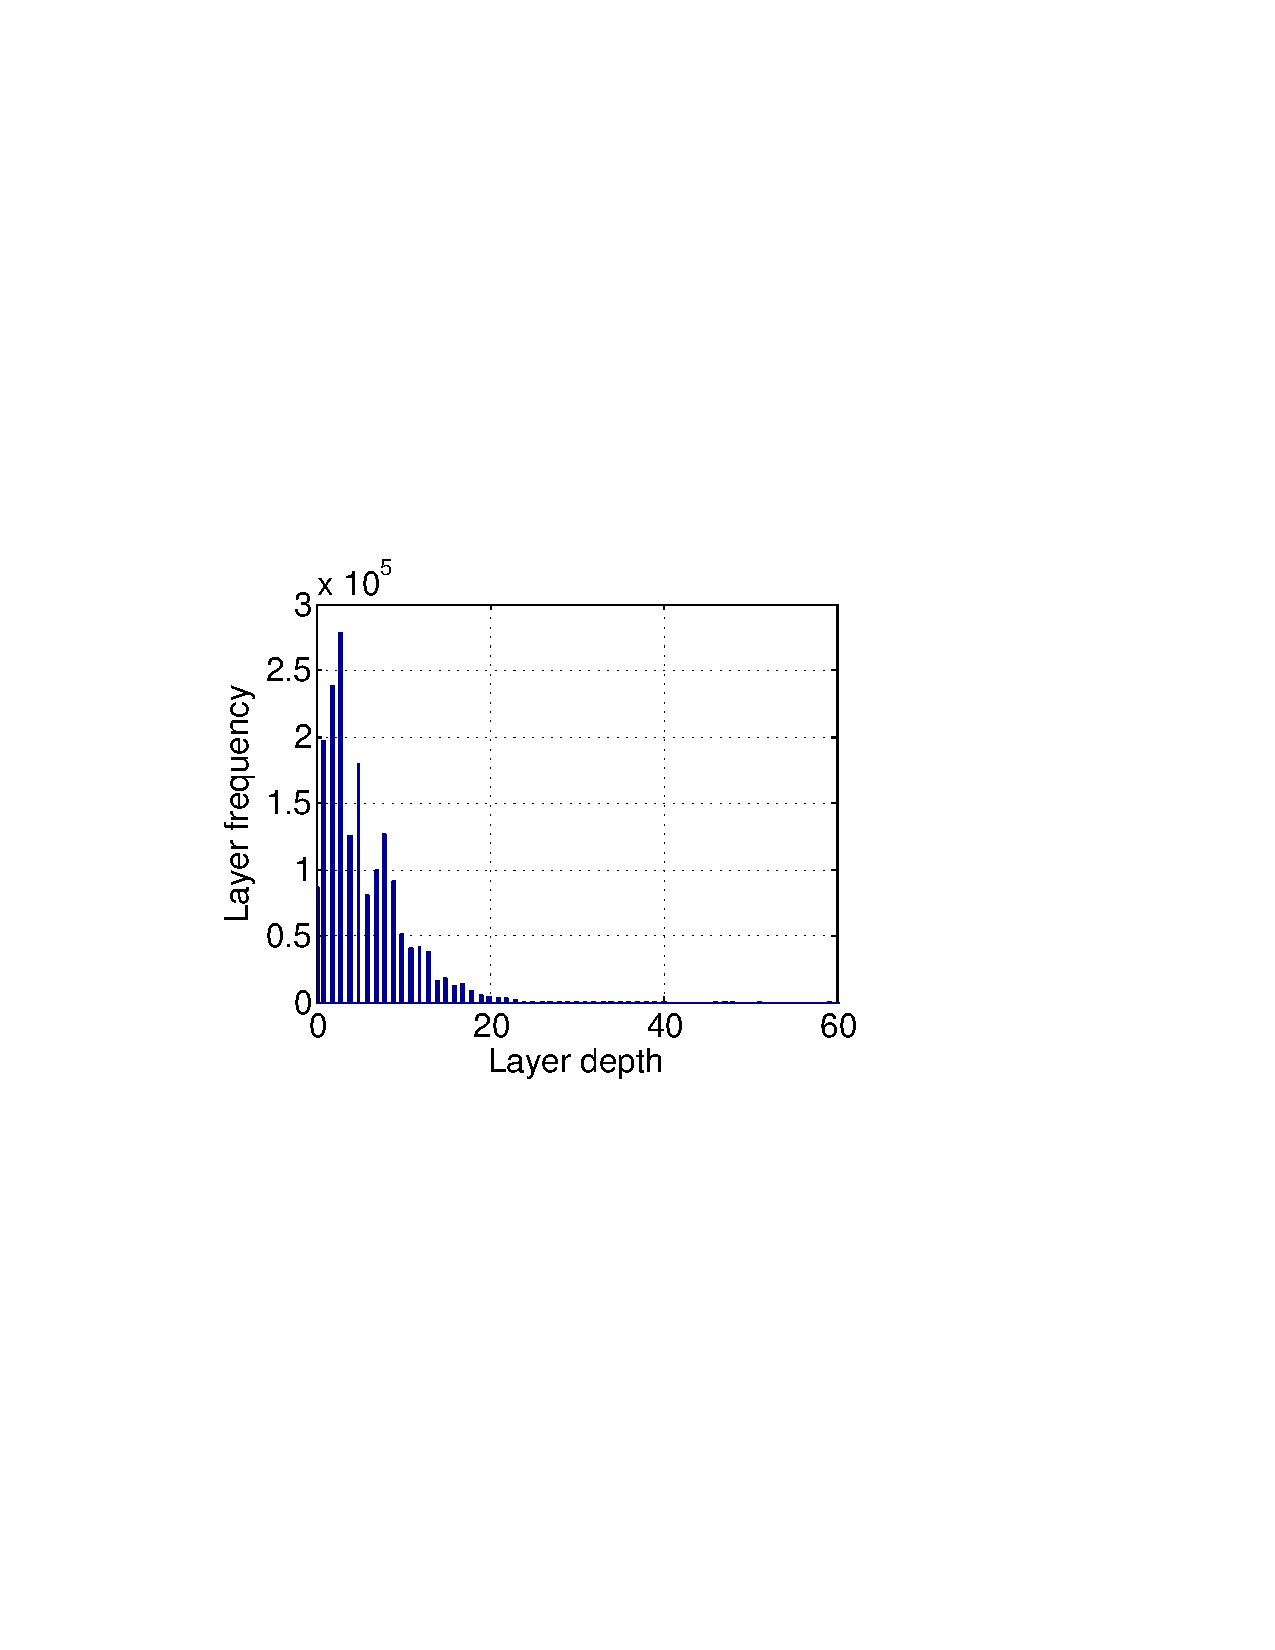
\includegraphics[width=0.21\textwidth]{graphs/layer-depth-pdf.pdf}
%	}
%	\caption{Layer depth distribution}
%	\label{fig:reference-cnt}
%\end{figure}

%Our size analysis reveals an interesting trade-off. Compression is
%computationally expensive and is one of the major sources of latency when
%pulling an image from Docker Hub~\cite{slacker}.  As the majority of layers is
%small and has low compression ratios, it can be beneficial to store small
%layers uncompressed in the registry to reduce pull latencies.

\paragraph{Directory count}

\begin{figure}[t]
	\centering
	\begin{minipage}{0.22\textwidth}
		\centering
		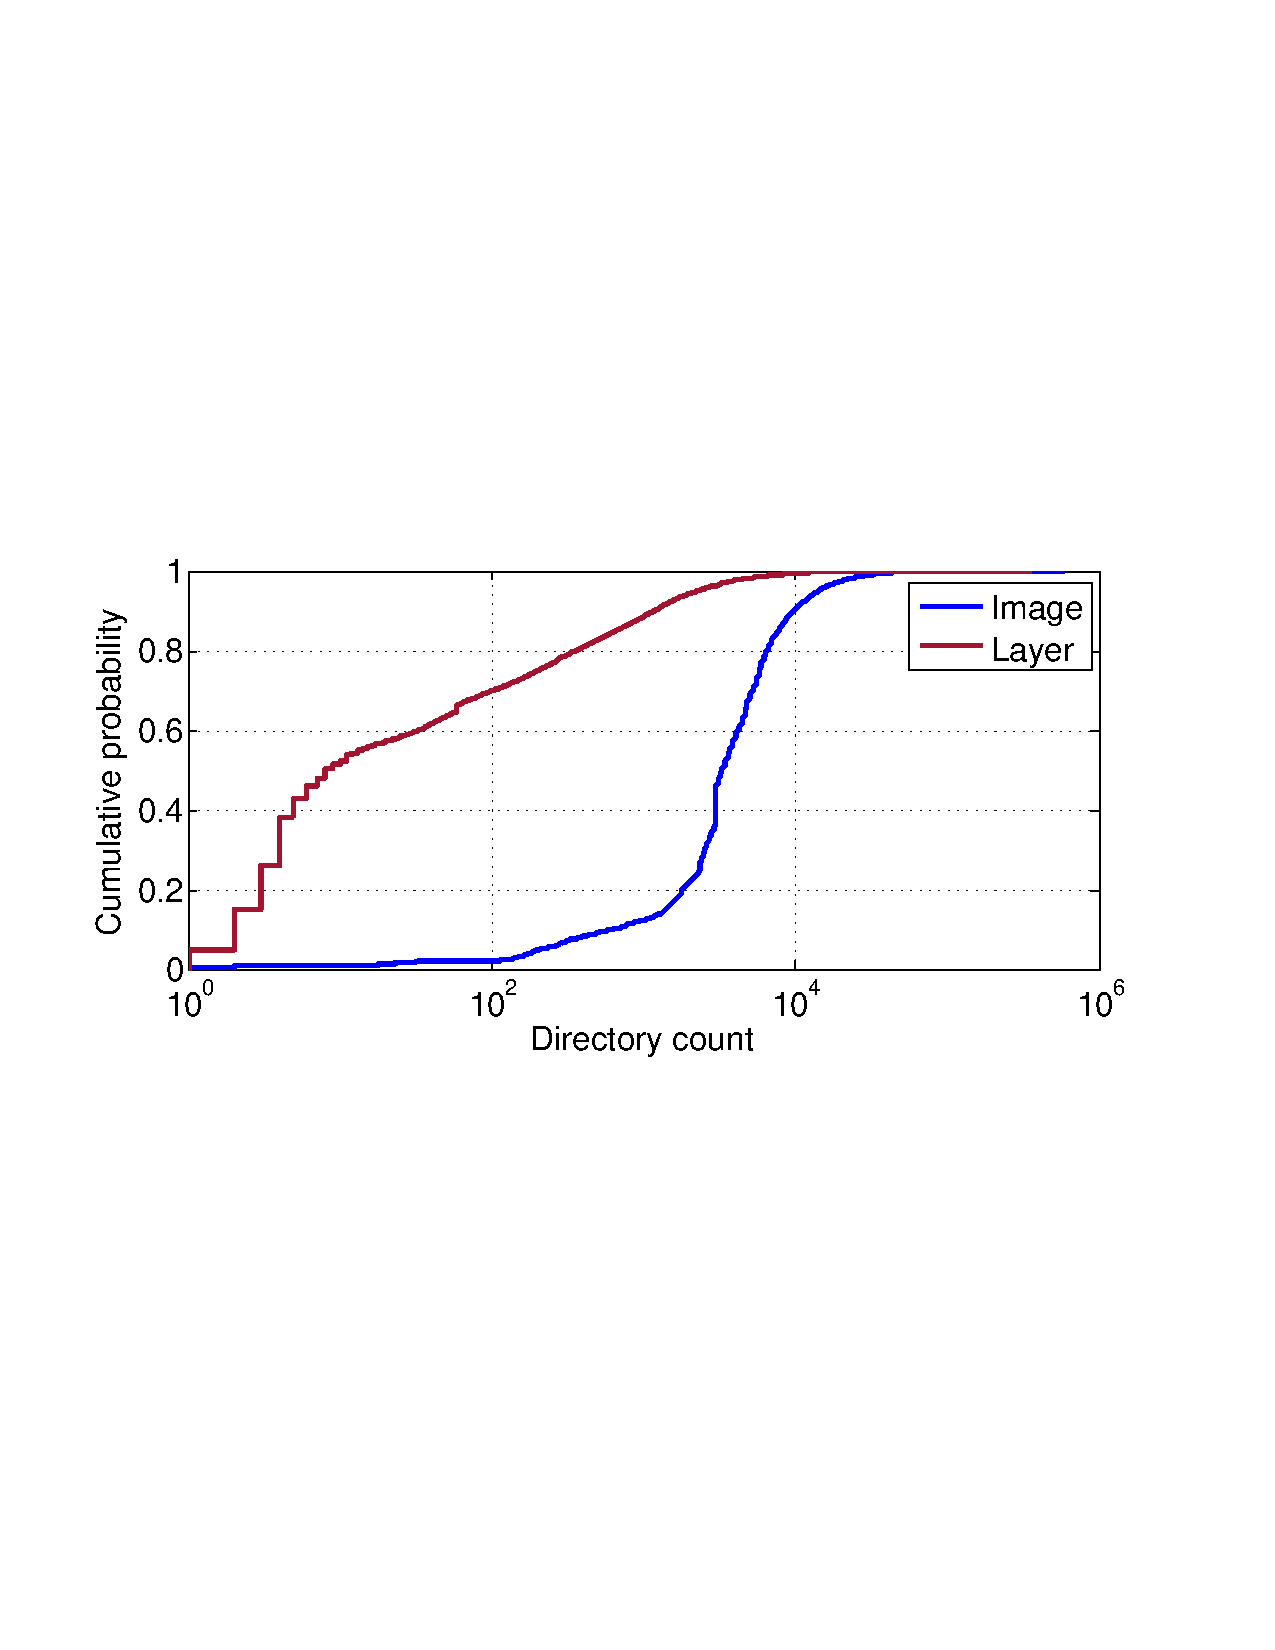
\includegraphics[width=1\textwidth]{graphs/dir-cnt-cdf.pdf}
		\caption{CDF of directory count}
		\label{fig:dir-cnt-cdf}
	\end{minipage}%
	\begin{minipage}{0.22\textwidth}
		\centering
		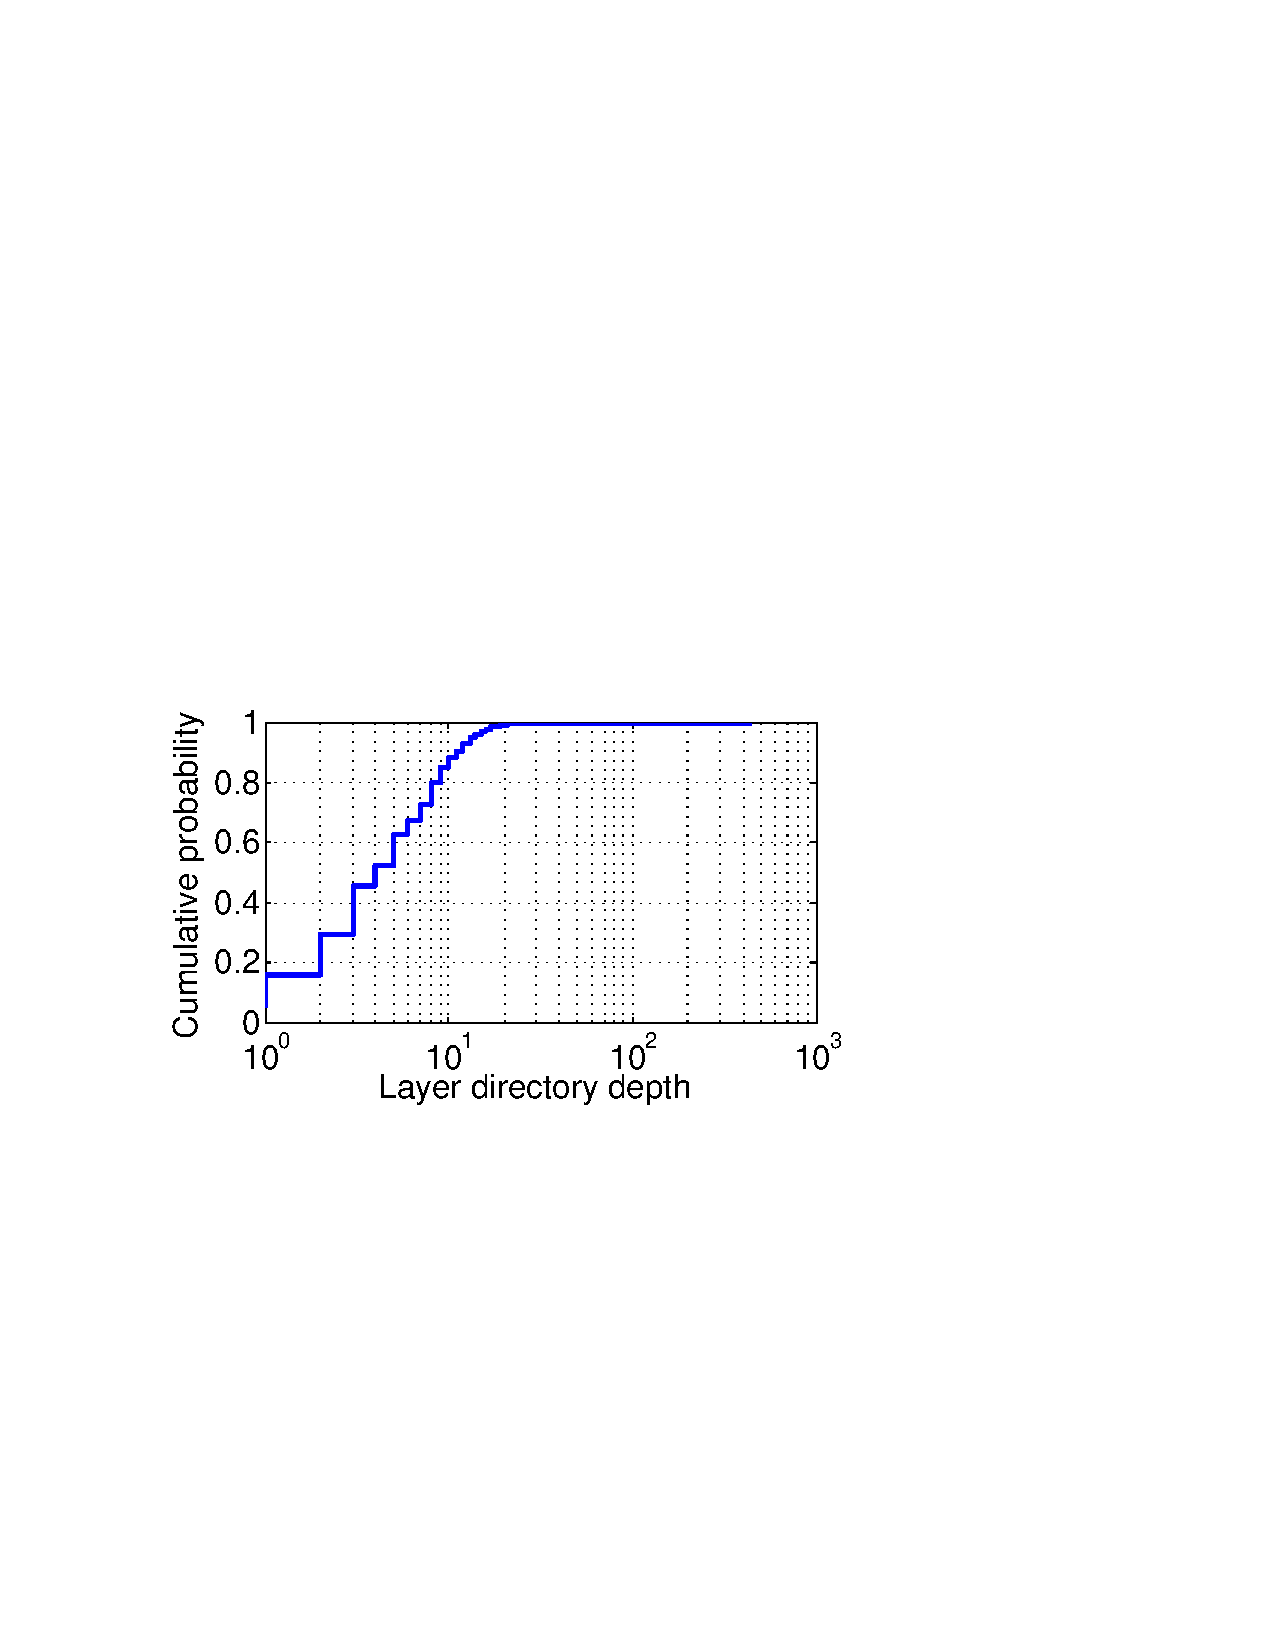
\includegraphics[width=1\textwidth]{graphs/layer-depth-cdf.pdf}
		\caption{CDF of layer directory depth}
		\label{fig:layer-depth-cdf}
	\end{minipage}
\end{figure}


Next, we look at the directory (Figure~\ref{fig:dir-cnt-cdf}), layer directory
depth(Figure~\ref{fig:layer-depth-cdf}) and file count
(Figure~\ref{fig:file-cnt-cdf}) in layers to determine if deploying images
requires handling of large amounts of metadata.

First looking at directories, we see that
%90\% of layers have less than 1,146 directories
70\% of layers have less than 100 directories and around 10\% of layers have
bigger than 1,000 directories while the median is at 8.
%
\emph{Majority of layers have a small number of directories while a small
number of layers contains large amount of directories, which might cause
metadata overhead for the underlying union file system.}
%For files, 90\% of images have less than 64,780 files with a median of 1,090.

\paragraph{Layer directory depth}

To further understand the metadata overhead, we decompressed the layer gzip
compressed archival file as a layer directory and counted the layer directory
depth as the maximum directory depth of its containing directories as shown in
Figure~\ref{fig:layer-depth-cdf}.
%
50\% of layers have less 4 levels in layer directory depth and 90\% of layers
have less than 11 levels.
%
\emph{Most of Layers have a moderate number of directory levels, which means
directory depth is not a big concern of Docker designer.}

\paragraph{File count}

%\nancomment{still metadata overhead}
%\begin{figure}
%	\centering
%	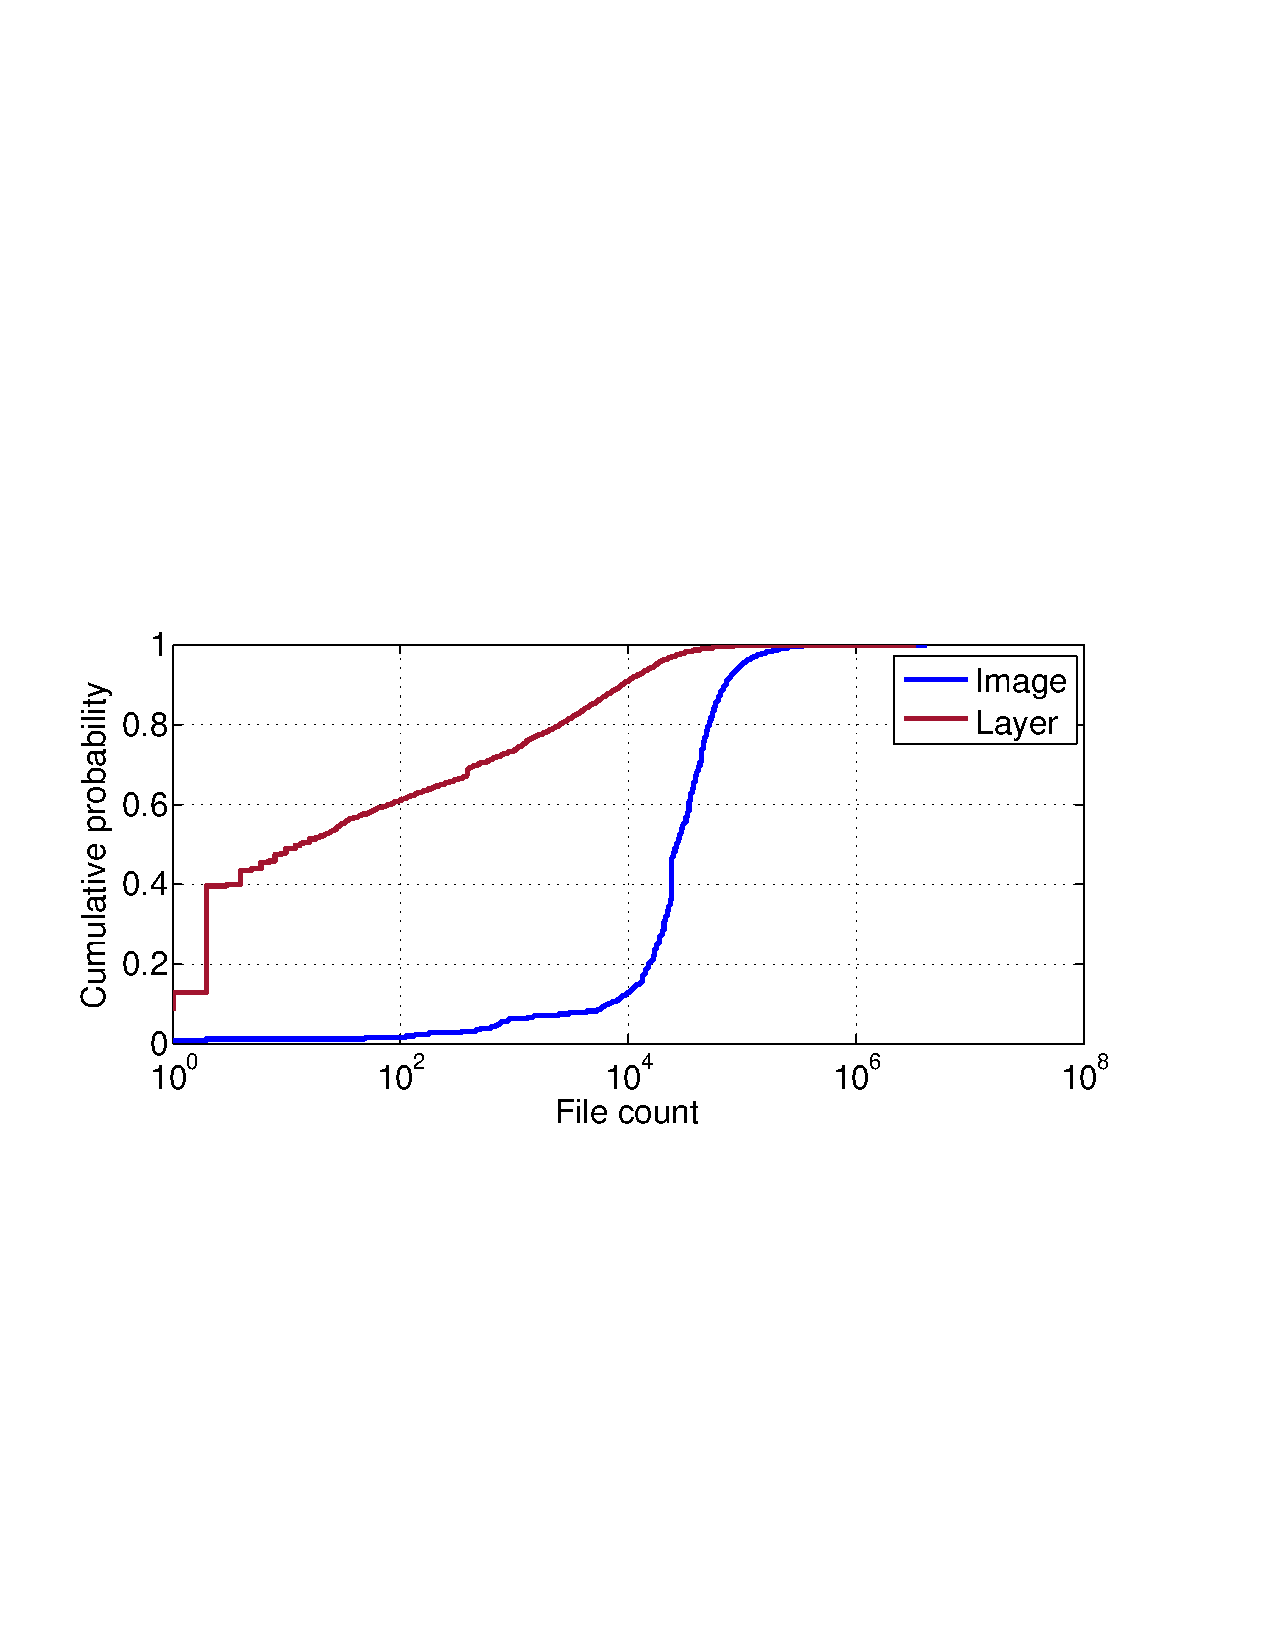
\includegraphics[width=0.4\textwidth]{graphs/file-cnt-cdf.pdf}
%	\caption{CDF of file count per image/layer.
%	}
%	\label{fig:reference-cnt}
%\end{figure}

%\begin{figure}[!t]
%	\centering
%	\subfigure[Histogram of directory count per image]{\label{fig_reference_cnt_cdf}
%		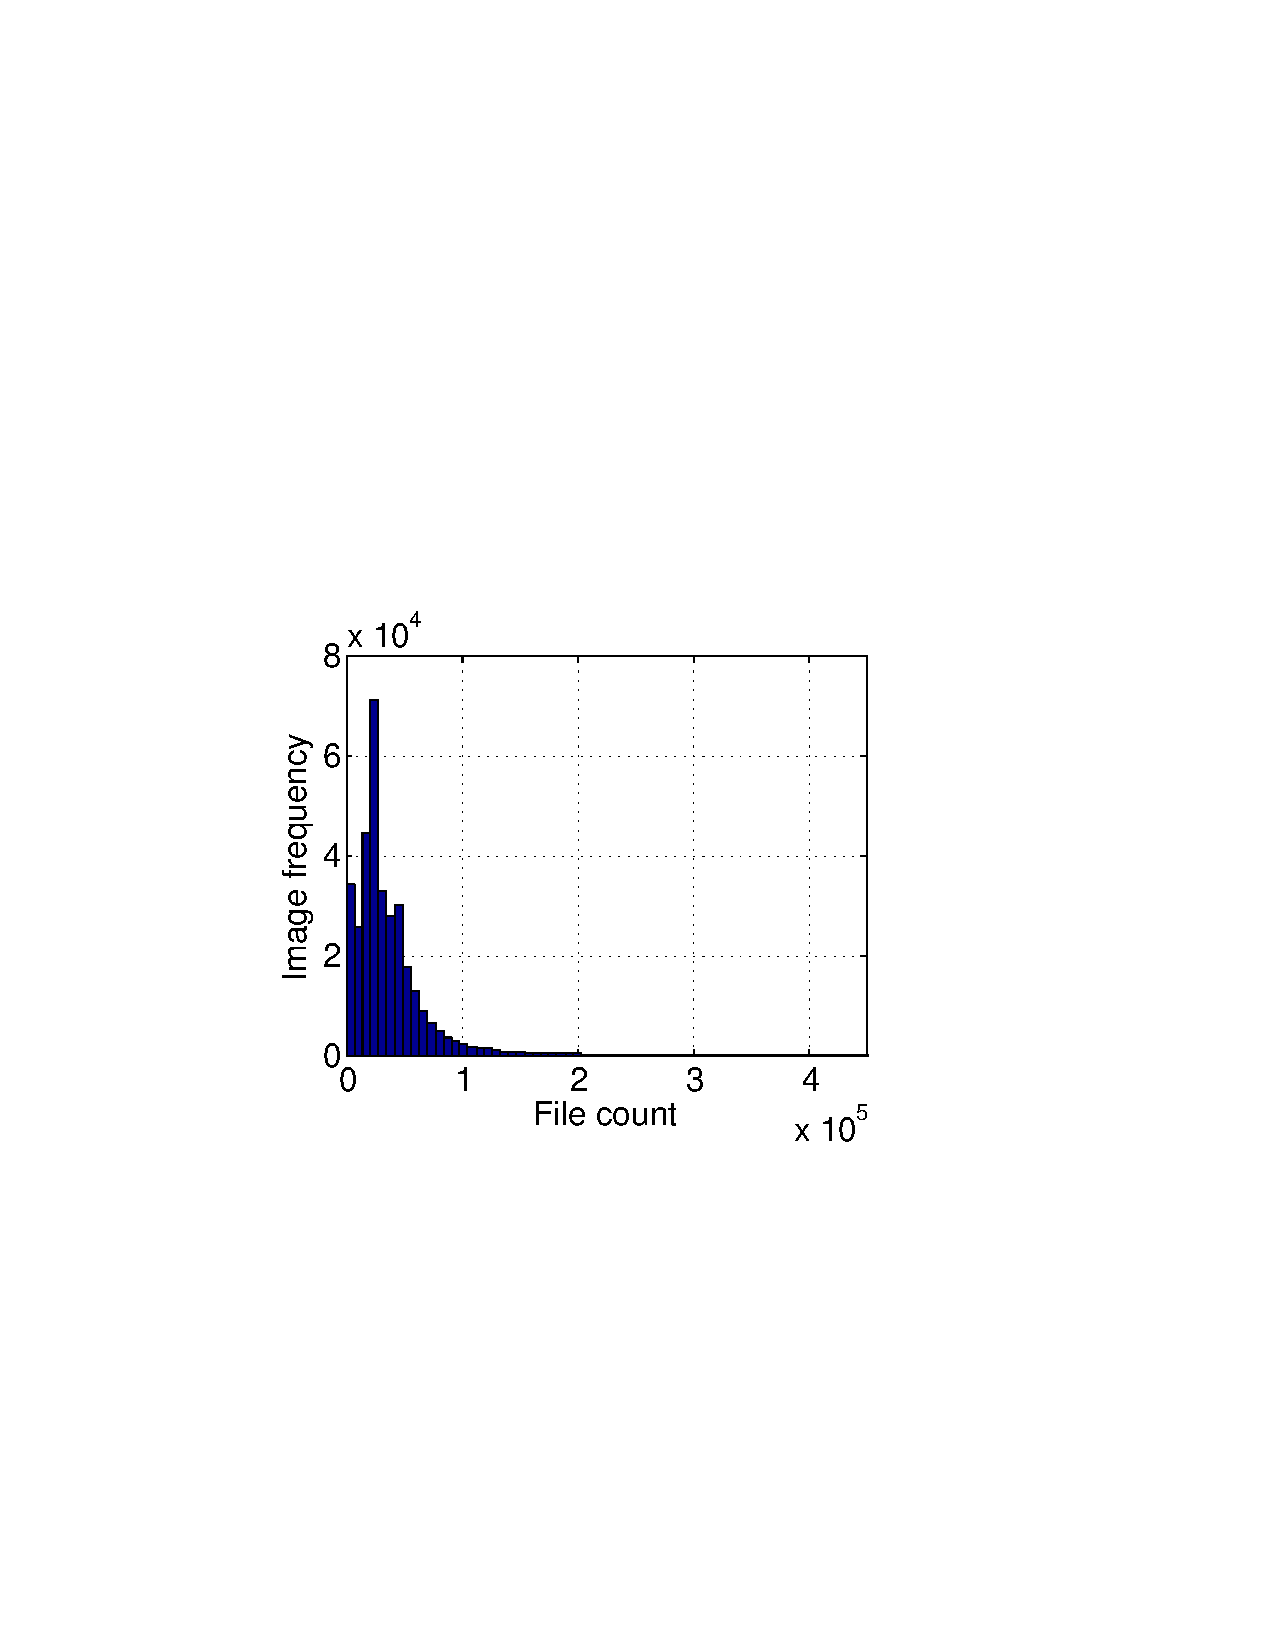
\includegraphics[width=0.21\textwidth]{graphs/image-file-cnt-pdf.pdf}%
%	}
%	\subfigure[Histogram of directory count per layer]{\label{fig_reference_cnt_pdf}
%		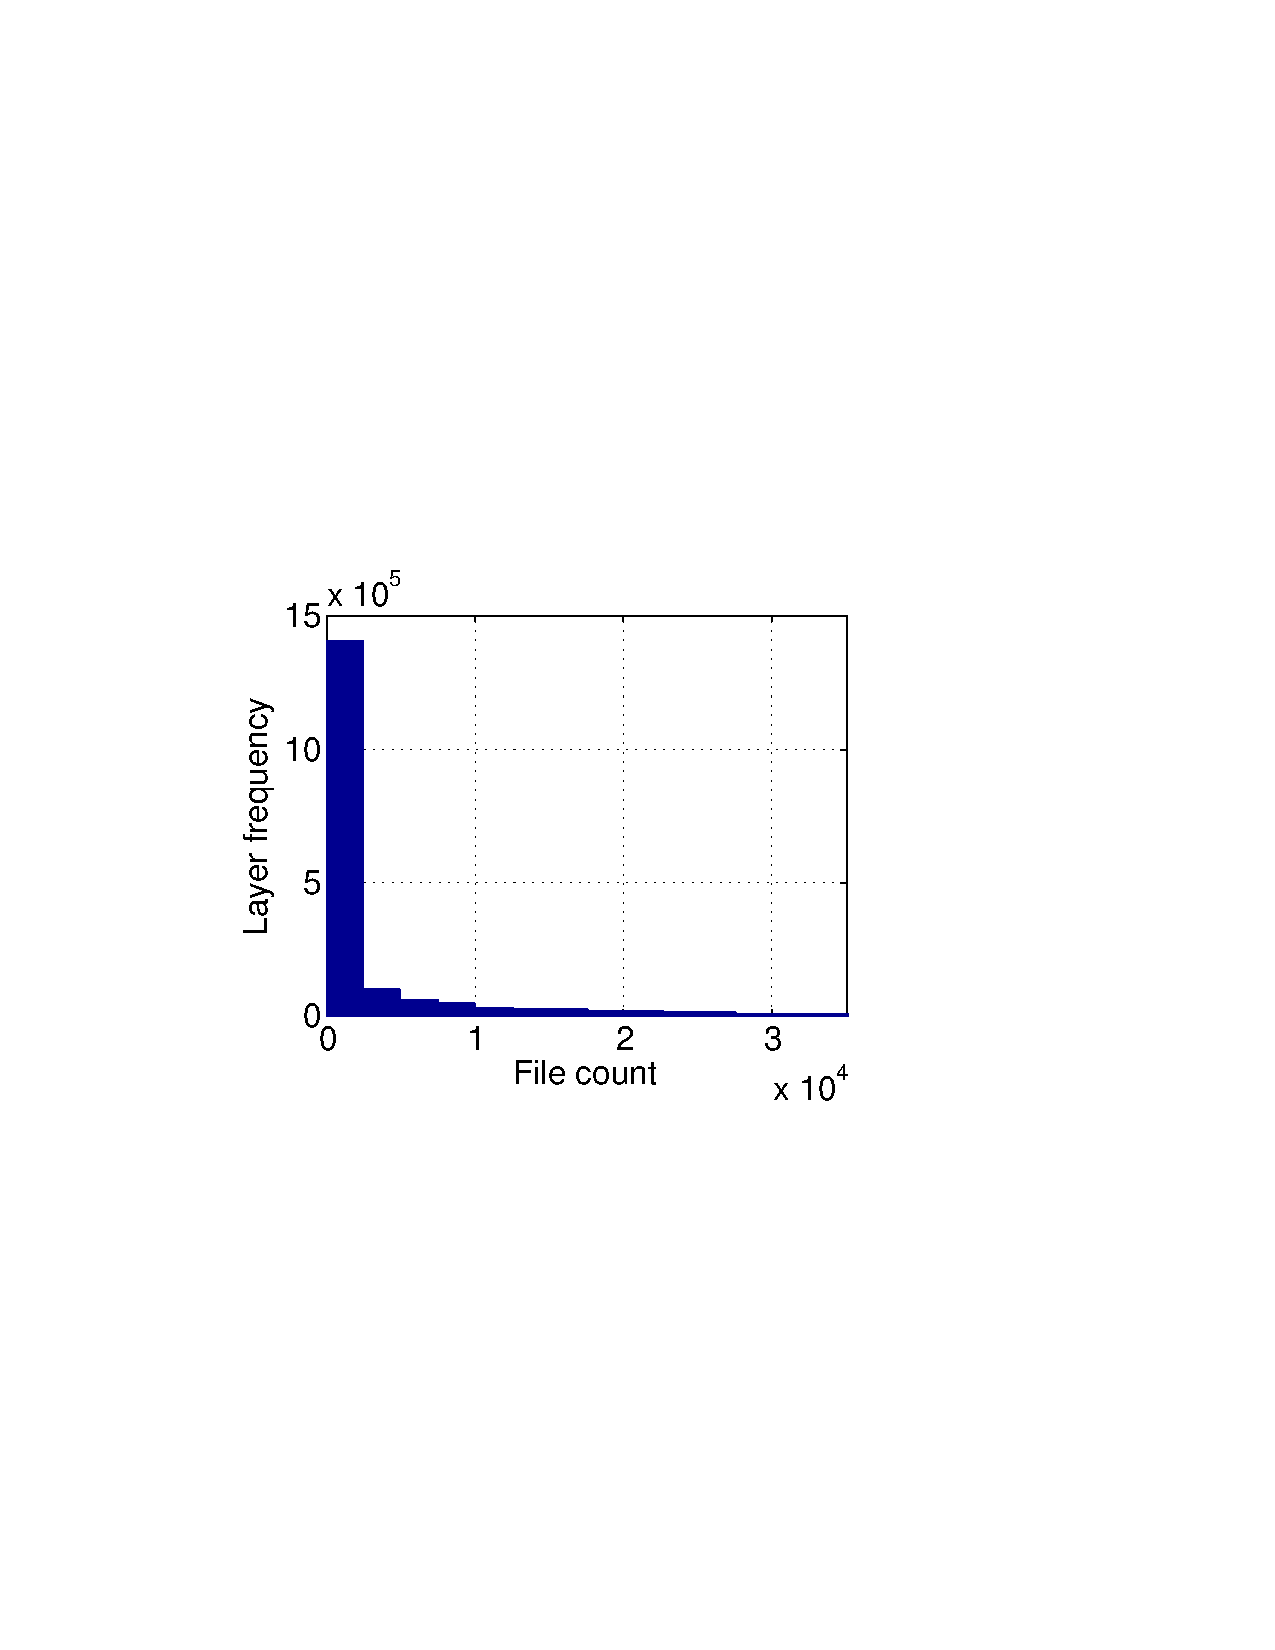
\includegraphics[width=0.22\textwidth]{graphs/layer-file-cnt-pdf.pdf}
%	}
%	\caption{Histogram of directory count distribution}
%	\label{fig:reference-cnt}
%\end{figure}

Lastly, we look at file count in layers as shown in
Figure~\ref{fig:file-cnt-cdf}.
%
%and directory metrics in layers.  and~\ref{fig_dir_cnt}
%Figure~\ref{fig:file-cnt-cdf} show the CDFs of file and directory counts in
%all layers, respectively.
%
The results show that 90\% of layers contain less than 9,467 files while half
of the layers have less than 12 files.
%50\% of layers have less 12 files and 90\% of images have           files
%
We also found that 13\% of the layers only have a single file.
%
30\% of layers have more than 600 files.
%
\emph{This analysis shows that the majority of layers consists only of a small
number of files and does not contain deeply nested directory hierarchies.
%
Hence, except a few outliers, unpacked layers do not require a large amount of
metadata from the storage system.}

% while 7\% even
%showed no files at all. We currently do not know the exact reason for the
%layers without files, but one theory is that these layers use Docker volumes to
%store all requred files (including executables).
% plan to investigate their corresponding images in the future.
%\nancomment{The layers are not empty since it could have directories}.
%On the other hand, the largest layer contains 826,196 files and was part of a
%Debian image.
%
%The average is 2,200.
%
%For directories, 90\% of the layers have less than 826 directories and half of
%the layers consist of less than 11 directories. We again observe a wide range
%with a minimum of a single directory and a maximum of 111,940. The layer with
%the most directories was part of the \emph{conjurinc/developer-quiz} image.

%\paragraph{Directory depths}

%After extracting and unpacking gzip compressed layer archival files,
%Besides the count, we also calculate the maximum directory depth for each layer
%(Figure~\ref{fig_layer_depth}).
%%
%Around 90\% of all layers have a directory depth less than 10 while for 50\% of
%the layers, the directory depth is less than 4.
%
%The most frequent directory depth is 3 with 313,000 layers showing this depth
%value (Figure~\ref{fig_hist_layer_depth}).
%
%About 313,000 layers' layer directory depth is 3, which is the peak value in
%the figure.
%
%The maximum repeat count is 444 while the median is 4. The average is ~5.
